\documentclass[dvipdfmx]{beamer}
\usepackage{etex}
%\documentclass[dvipdfmx,usenames]{beamer}
\usepackage{graphicx}
\usepackage{color}
\usepackage{listings}
\usetheme{Madrid}
\useinnertheme{circles}
\useoutertheme{default}
%\usepackage{beamerthemeshadow}
\usepackage{tikz}
\usepackage[varg]{txfonts}
\usepackage{booktabs}
\renewcommand{\kanjifamilydefault}{\gtdefault}
\setbeamercovered{transparent}
\setbeamertemplate{navigation symbols}{}
\everymath{\displaystyle}
\AtBeginSection[]
{\begin{frame}{発表の流れ}
	\begin{multicols}{2}[]
  \tableofcontents[currentsection]
	\end{multicols}
\end{frame}}
%ページ番号の表示
%\setbeamertemplate{footline}[frame number]
\usepackage{hyperref}
%しおりをつくるsectionの深さや,目次のリンクの色などを指定
%\usepackage[bookmarksopenlevel=2]{hyperref}
\usepackage{pxjahyper}
%amsmathとhyperrefとの互換性
\usepackage{amsmath}
\let\equation\gather
\let\endequation\endgather

\setbeamertemplate{enumerate item}[circle]

\newcommand{\backupbegin}{
  \newcounter{framenumberappendix}
  \setcounter{framenumberappendix}{\value{framenumber}}
}
\newcommand{\backupend}{
  \addtocounter{framenumberappendix}{-\value{framenumber}}
  \addtocounter{framenumber}{\value{framenumberappendix}}
}

%\lstset{
%	language= C,
%	numbers=left,		numbersep= 10pt,		numberstyle= \ttfamily,
%	breaklines=ture,	breakindent= 20pt,
%	%frame= shadowbox,	
%	framesep= 3pt,	rulesep= 4pt,
%	stepnumber= 1,
%	backgroundcolor= \color{white},
%	rulesepcolor= \color{cyan},
%	basicstyle= \ttfamily, %columns= [1][fullflexible],
%	tabsize=2,
%	label= %
%}

\lstdefinestyle{customc}{
	belowcaptionskip=1\baselineskip,
	breaklines=true,
	frame=L,
	xleftmargin=\parindent,
	language=C,
	showstringspaces=false,
	%basicstyle=\footnotesize\ttfamily,
	basicstyle=\tiny\ttfamily,
	keywordstyle=\bfseries\color{green!40!black},
	commentstyle=\itshape\color{purple!40!black},
	identifierstyle=\color{blue},
	stringstyle=\color{orange},
	tabsize=2,
}

\lstdefinestyle{customasm}{
	belowcaptionskip=1\baselineskip,
	frame=L,
	xleftmargin=\parindent,
	language=[x86masm]Assembler,
	basicstyle=\footnotesize\ttfamily,
	commentstyle=\itshape\color{purple!40!black},
}
\lstset{escqpechar=@,style=customc}


\usepackage{subcaption}
\usepackage{multicol}
\usepackage{lmodern}
\usepackage{advdate}

\title[数値アルゴリズム特論]{Lecture 5. More on the SVD}
\institute{Kogakuin University}
\author[Shota Tsuji]{情報学部コンピュータ科 j114081 辻 祥太}
%\date{\AdvanceDate[1]\today}
\date{\today}


\begin{document}
\section*{はじめ}
\begin{frame}
  \titlepage \end{frame} 
\begin{frame}[plain]
  \frametitle{Contents}
  \tableofcontents
\end{frame}

\begin{frame}
  \frametitle{Contents}
	%\begin{multicols}{2}[]
  \begin{itemize}
    \item 行列行列積の計算
    \item 実測性能の確認
  \end{itemize}
	%\end{multicols}
\end{frame}

\section{行列行列積の計算}
\begin{frame}
  \frametitle{課題の指定}
  指定された条件
  \begin{enumerate}
		\item N*Nの正方行列の積$(100\leq N \leq 1000)$
		\item 演算時間を計算
  \end{enumerate}
\end{frame}


\begin{frame}
	\frametitle{Aluminium(Intel Xeon X5570)}
	\begin{columns}
	\begin{column}{0.48\textwidth}
	\begin{itemize}
		\item Frequency 2.93[GHz]
		\item cache\_size 8192 KB
		\item 1Clockあたりの演算回数\\ 2[Flops/Clock]
	\end{itemize}

	\begin{itemize}
		\item \$ cat /proc/cpuinfo で確認できる
	\end{itemize}
	\end{column}

	\begin{column}{0.48\textwidth}
	\begin{figure}
	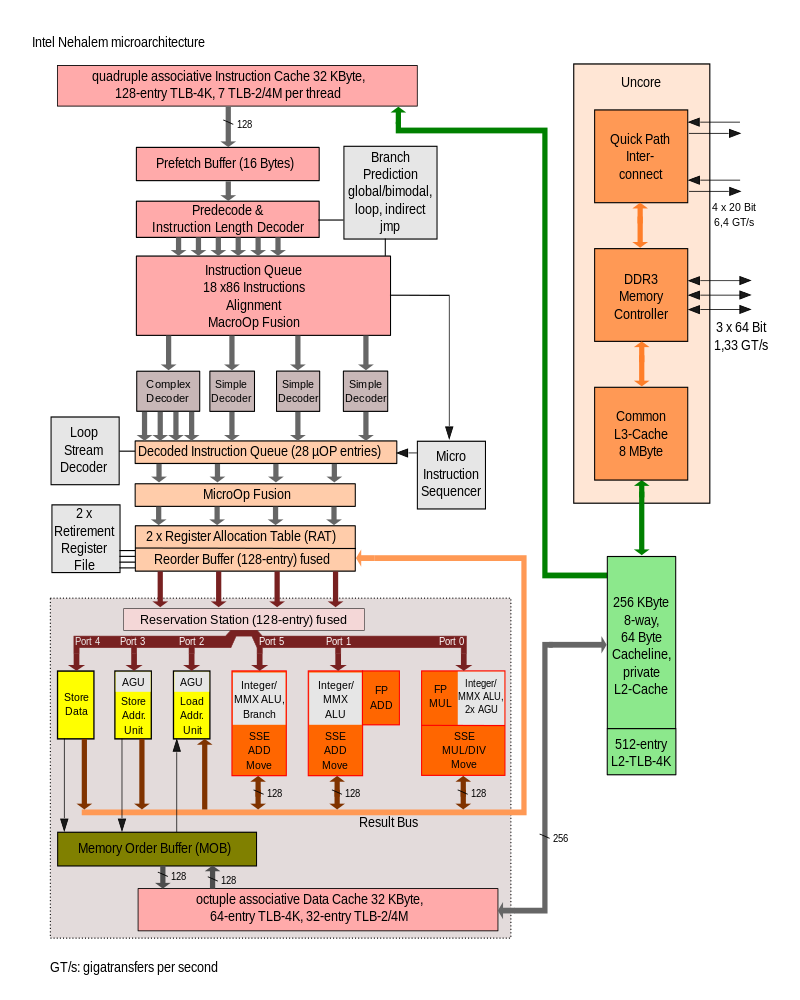
\includegraphics[width=0.5\paperwidth, natwidth=910,natheight=940]{./800px-Intel_Nehalem_arch.svg.png}
	\end{figure}
	\end{column}
	\end{columns}
\end{frame}

\section{性能値の計算}
\begin{frame}
  \frametitle{性能値の計算}
	\begin{block}{理論性能値}
	\begin{equation*}
		%(\mbox{性能値GFlops}) = (\mbox{1Clockあたりの演算回数}) * (\mbox{Frequency}) * (\mbox{コア数}) \\
		(GFlops) = (FLOPS/Clock) * (Frequency) * (Num\_Cores)
  \end{equation*}
	\end{block}

	\begin{block}{実測性能値}
	\begin{center}
  \begin{equation*}
		(\mbox{GFlops}) = \frac{(\mbox{計算1回あたりの演算回数})*(\mbox{計算回数})}{(\mbox{全体で掛かった時間)*($10^9$)}}
  \end{equation*}
	\end{center}
	\end{block}
	Flopsとは,1秒あたりの演算回数(Flop/sec)\\
	Aluminium計算機での理論値
	\begin{equation*}
		2 * 2.93 * 1 = 5.86GFlops
  \end{equation*}
\end{frame}


%\begin{frame}
 % \frametitle{使用した計算機の特徴と実行環境}
 % \begin{columns}
 % \begin{column}{0.48\textwidth}
 % \begin{itemize}
 % 		\item コンパイル\\ gcc -fopenmp sem\_mat\_mat.c -lm
 % 		\item コアは1個のみ使用
 % \end{itemize}
 % \end{column}

 % \begin{column}{0.48\textwidth}
 % \begin{table}
 %   \caption{Aluminium計算機}
 % 	\centering
 %   \begin{tabular}{ c | r } \toprule
 % 		特徴 & 内容\\ \midrule
 %     種類 & Intel Xeon X5570\\
 %     コア数 & 2コアまで\\
 % 		周波数 & 2.93GHz\\ \bottomrule
 %   \end{tabular}
 % \end{table}
 % \end{column}
 % \end{columns}
%\end{frame}


%\begin{frame}
 % \frametitle{性能値の計算}
 % \begin{equation*}
 % 	(\mbox{性能値GFlops}) = (\mbox{1Clockあたりの演算回数}) * (\mbox{Frequency}) * (\mbox{コア数})
% \end{equation*}
%\end{frame}

\section{実行とコード内容}
\begin{frame}
	\frametitle{Execution}
	\begin{columns}
	\begin{column}{0.60\textwidth}
	Command
	Content of script
	\end{column}
	\begin{column}{0.30\textwidth}
	\begin{itemize}
		\item shell scriptで行列の大きさNを変えながら回す\\
		\item 刻み幅は50\\
		\item result???.csvに書き込む
	\end{itemize}
	\end{column}
	\end{columns}
\end{frame}

\begin{frame}
	\frametitle{Sorce Code of sem\_mat\_mat.c}
	\begin{columns}
	\begin{column}{0.60\textwidth}
		時間計測
	\end{column}
	\begin{column}{0.30\textwidth}
		omp\_get\_wtime()を使う
		行列Cへの値を足しこむ部分を囲む
	\end{column}
	\end{columns}
\end{frame}


\begin{frame}
	\frametitle{考察}
	愚直な行列行列積(2次元配列の場合)
	\begin{itemize}
		\item 行列bに対し,列方向でアクセスしている\\ 空間的局所性を考えていないプログラム
	\end{itemize}
	%double型のサイズは,8byte
\end{frame}

\begin{frame}
	\frametitle{これからすること}
	\begin{itemize}
	\item 行列を1次元でとる
	\item 最適化オプション試してみる
	\end{itemize}
\end{frame}

% codeのサイズを小さめにする
% 式の番号表示しない
% 1次元配列にしたときの計算
% サイズ/timeの結果
% 理論性能との比較
% コンパイルオプションつき
% adressen あドレッセん
% よこせん(スライド一枚を分割)
\appendix
\backupbegin

\begin{frame}
  \begin{center}
    \huge appendixes
  \end{center}
\end{frame}

\begin{frame}
  \frametitle{使用した計算機の特徴と実行環境}
	\begin{columns}
	\begin{column}{0.48\textwidth}
	\begin{itemize}
			\item コンパイル\\ gcc -fopenmp sem\_mat\_mat.c -lm
			\item コアは1個のみ使用
	\end{itemize}
	\end{column}

	\begin{column}{0.48\textwidth}
  \begin{table}
    \caption{Aluminium計算機}
		\centering
    \begin{tabular}{ c | r } \toprule
			特徴 & 内容\\ \midrule
      種類 & Intel Xeon X5570\\
      コア数 & 2コアまで\\
			周波数 & 2.93GHz\\ \bottomrule
    \end{tabular}
  \end{table}
	\end{column}
	\end{columns}
\end{frame}


\begin{frame}
%  \frametitle{参考文献}
%  \begin{thebibliography}{9}
%    \bibitem{pca_start}
%    統計学研究所 www.statistics.co.jp/reference/software\_R/statR\_9\_principal.pdf
%    \bibitem{knn}
%    http://machinelearningmastery.com/tutorial-to-implement-k-nearest-neighbors-in-python-from-scratch/
%  \end{thebibliography}
\end{frame}

\backupend
\end{document}
